%% beamerthemeImperialPoster v1.0 2016/10/01
%% Beamer poster theme created for Imperial College by LianTze Lim (Overleaf)
%% LICENSE: LPPL 1.3
%%
%% This is the example poster demonstrating use
%% of the Imperial College Beamer Poster Theme
\documentclass[xcolor={table}]{beamer}
%% Possible paper sizes: a0, a0b, a1, a2, a3, a4 (although Imperial College posters are usually A0 or A1).
%% Possible orientations: portrait, landscape
%% Font sizes can be changed using the scale option.
\usepackage[size=a0,orientation=portrait,scale=1.55]{beamerposter}
\usepackage{algorithm}
\usepackage{algpseudocode}
\usepackage{multirow}
\usepackage{graphicx}
\usepackage{subcaption}

\usetheme{ImperialPoster}

%% Four available colour themes
\usecolortheme{ImperialWhite} % Default
% \usecolortheme{ImperialLightBlue}
% \usecolortheme{ImperialDarkBlue}
% \usecolortheme{ImperialBlack}

\title{Smart-CPR: Self-Organisation and Self-Governance \newline in the Sharing Economy}



\author{David Burth Kurka and Jeremy Pitt}

\institute{Department of Electrical and Electronic Engineering, Imperial College London}

% \addbibresource{sample.bib}


\begin{document}

\begin{frame}[fragile=singleslide,t]\centering

\maketitle

\begin{columns}[onlytextwidth,T]

%%%% First Column
\begin{column}{.48\textwidth}

\begin{block}{Distributed Resource Allocation - $LPG'$}

\begin{itemize}
\item Producers independently operate in a market of common manufactured widgets
\item Over time, producers receive demands for products ($q$) and keep a capacity of production output ($g$)
\item Producers cooperate by distributing offer ($p$) and demand ($d$) in a common pool of services
\item Resources of industrial supply and demand are distributed ($r$) among producers, following stipulated rules
\end{itemize}

\begin{figure}
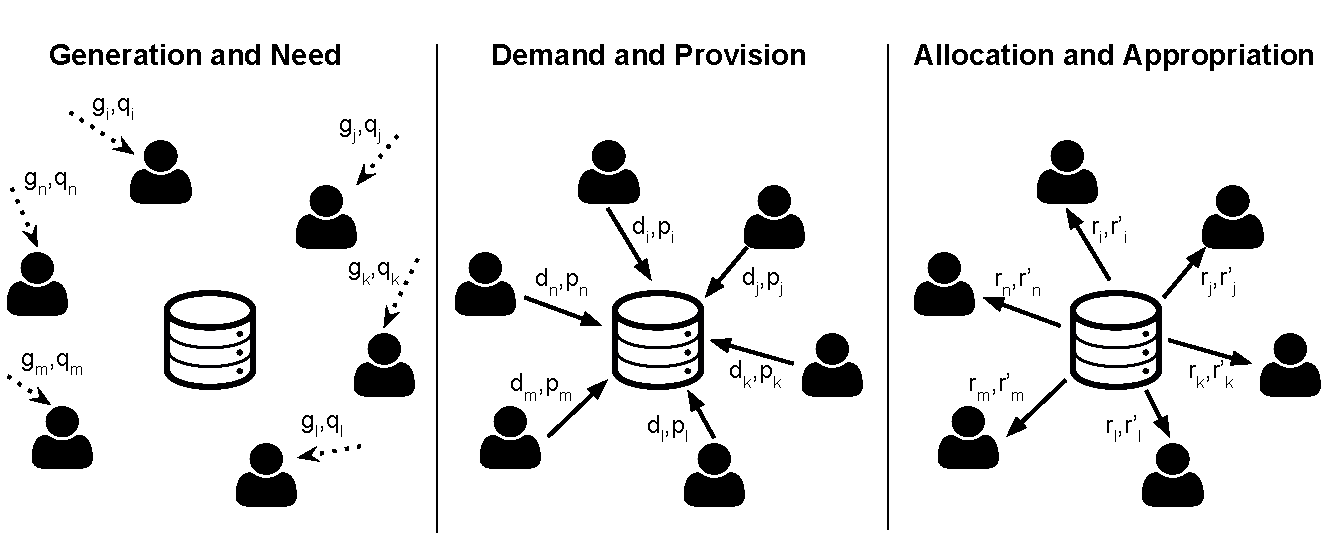
\includegraphics[width=\linewidth]{pics/lpg.pdf}
\end{figure}

\end{block}


\begin{block}{Questions}
\begin{itemize}
\item How to ensure \textbf{efficient, fair, inclusive and sustainable}
ways to distribute services among producers?
\item What \textbf{rules and norms} should
govern the interactions and transactions?
\item \textbf{Who} should determine the
stipulated rules? 
\item How to deal with \textbf{abuses} and \textbf{non-compliance} with the rules?

\end{itemize}
\end{block}


\begin{block}{Actors Model: Smart-CPR}
\begin{figure}
\centering
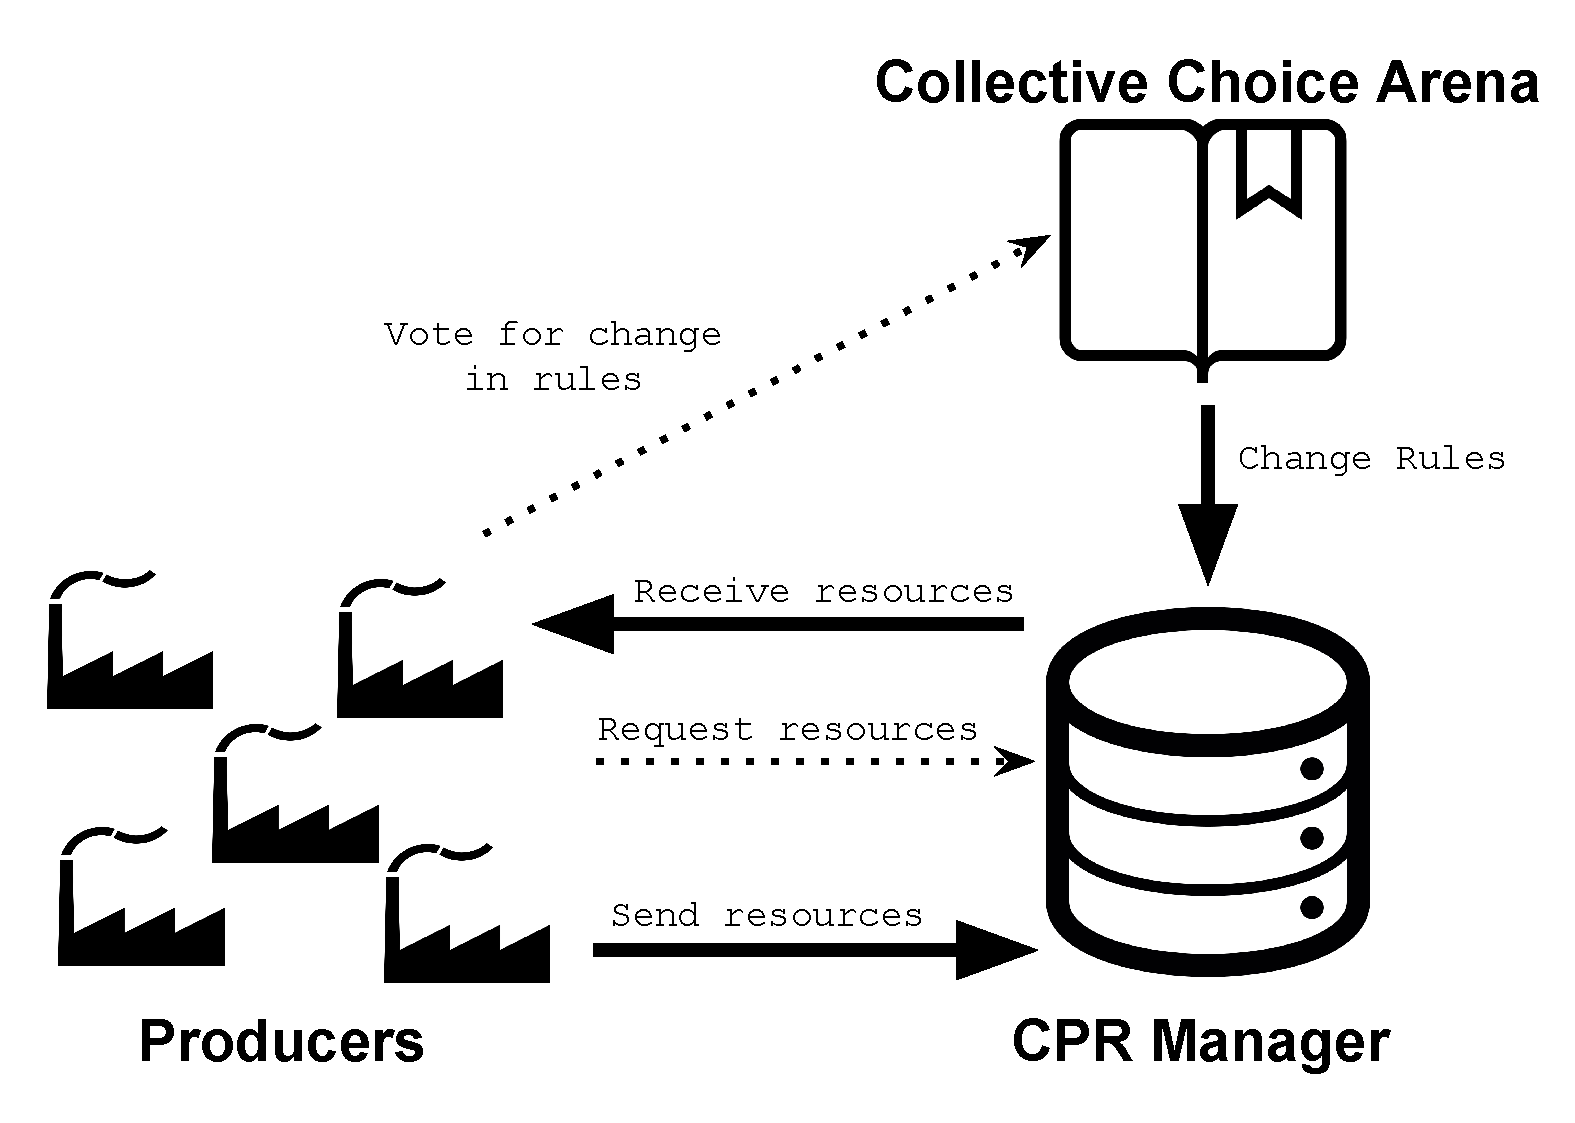
\includegraphics[width=0.7\linewidth]{pics/smartpool_ind.pdf}
%\caption{Diagram representing Smart-CPR system model with interactions between the system's actors.}\label{fig:diagram}
\end{figure}


\underline{\textbf{Producer}}
\begin{itemize}
    \item Responsible for mediating provision and demands of resources to the CPR Manager
    \item Participant of the Collective Choice Arena, being able to cast votes and update CPR Manager's policies to it's own benefit
\end{itemize}

\underline{\textbf{CPR Manager}}

\begin{itemize}
    \item Responsible for fast decision making of resource allocation
    \item Smart-Contract define policy and rules for responses for resources request
    \item Blockchain ledger stores producers participation and behaviour
\end{itemize}

\underline{\textbf{Collective Choice Arena}}

\begin{itemize}
    \item Compute producers' votes for change on CPR Manager rules
    \item Issue new smart-contracts to be used as policy for CPR Manager
\end{itemize}



\end{block}

\end{column}


%%%% Second Column
\begin{column}{.48\textwidth}


\begin{block}{Policy Making - Smart-Contract}

Rescher's legitimate claims of justice is used as metric to evaluate producer participation in the system (according to the public ledger): 

\begin{table}
\renewcommand{\arraystretch}{1}
\color{black}
\small
\centering
% \caption{Legitimate claims of justice.}
\label{claims}
\begin{tabular}{|l|l|}
\hline
\multicolumn{1}{|l|}{\multirow{2}{*}{Canons of equality}} &  $\phi_{i}^{1} = R_i$ \\ \cline{2-2} 
\multicolumn{1}{|l|}{}                               &  $\phi_{i}^{2} = 
                                                          \begin{cases} 
                                                          (1 - \alpha) \cdot \phi_{i}^{2} +  \alpha & \text{if accepted req.}\\
                                                          (1 - \beta) \cdot \phi_{i}^{2} & \text{if denied req.}
                                                        \end{cases}$ \\ \hline
Canon of needs                                       &  $\phi_{i}^{3} = D_i$ \\ \hline
Canon of productivity                                &  $\phi_{i}^{4} = P_i$ \\ \hline
Canon of effort                                      &  $\phi_{i}^{5} = \mathit{CurTime} - \mathit{JoiningTime}$ \\ \hline
  Canon of social utility                              &  $\phi_{i}^{6} = \mathit{Status}(i)$\\ \hline
\end{tabular}
\end{table}



\renewcommand{\algorithmicrequire}{\textbf{Require:}}

\algrenewcommand\algorithmicprocedure{\textbf{Smart-contract}}

Upon a request for resource, a weighted sum of the claims is computed and a response is evaluated based on a smart-contract policy:

\begin{center}
\begin{minipage}{0.8\textwidth}
\begin{algorithm}[H]
  \footnotesize
\renewcommand\thealgorithm{}
\caption{Smart-Contract}\label{smartcontract}
\begin{algorithmic}[0]
\Require 
\State $W = [w_1, w_2 \dots w_n]$\Comment{Weights for different claims}
\State $S_t$\Comment{Score Threshold}

\Statex
\Procedure{EvaluateRequest}{}%{$UserId, Request, Ledger$}
\State $\Phi_i = [\phi^1_i, \phi^2_i \dots \phi^n_i] \gets \Call{getMerit}{\mathit{Ledger}, \mathit{UserId}}$
\State $S_i = \sum_{j=1}^{|C|} \left ( w_j * \phi_{i}^{j} \right)$
\If{$S_i \geq S_t \land \mathit{Pool} \geq \mathit{Request}$}
    \State \textbf{return} $\textit{accepted}$
\Else
    \State \textbf{return} $\textit{denied}$
\EndIf
\EndProcedure
\end{algorithmic}
\end{algorithm}
\end{minipage}
\end{center}


\end{block}

\begin{block}{Results}

Experiments observe two scenarios: (a) homogeneous full compliant populatoin and (b) a mix of compliant and non-compliant agents. %(i.e.\ non-cooperative) agents.
\end{block}

\begin{block}{Canon's weights self-organisation}

\begin{figure}
%  \caption{Weights progression in full compliance case.}\label{weightsexp0}
\centering

\begin{subfigure}[b]{0.48\linewidth}
    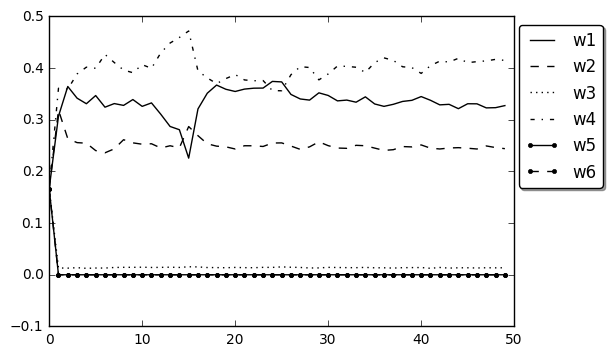
\includegraphics[width=\linewidth]{pics/weights_exp0_lc.png}
    \caption{Full compliant case}
\end{subfigure}
~%
\begin{subfigure}[b]{0.49\linewidth}
    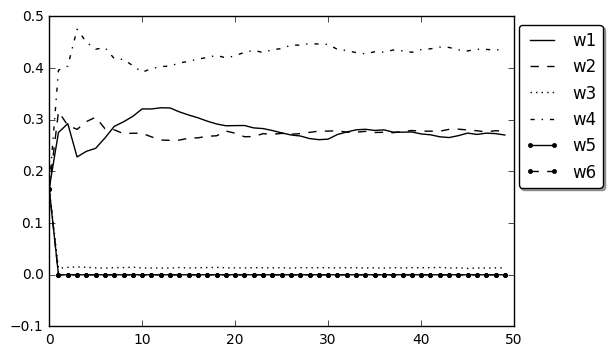
\includegraphics[width=\linewidth]{pics/weights_exp1_lc.png}
    \caption{Mixed population case}
\end{subfigure}
\end{figure}

\begin{itemize}
    \item Agents are able to self-organise the relevance of weights in order to benefit the majority of the network
\end{itemize}

\end{block}

\begin{block}{Resource Distribution Results}

\begin{table}[]
\color{black}
\small
\centering
% \caption{My caption}
\label{my-label}
\begin{tabular}{l|l|ll|}
\cline{2-4}
                                                & \multicolumn{1}{c|}{\textbf{Scenario A}} & \multicolumn{2}{c|}{\textbf{Scenario B}}     \\
                                                & Full Compliance                          & Compliant Agents     & Non Compliant         \\ \hline
\multicolumn{1}{|l|}{\textbf{Physical Facts}}   &                                          &                      &                       \\
\multicolumn{1}{|l|}{Demand}                    & $4096.49 \pm 14.24$                      & $4090.10 \pm 23.12$  & $4096.40 \pm 8.87$    \\
\multicolumn{1}{|l|}{Accrued}                   & $2730.12 \pm 18.00$                      & $3864.74 \pm 48.35$  & $454.72 \pm 14.71$    \\
\multicolumn{1}{|l|}{Generated}                 & $2730.17 \pm 17.85$                      & $2726.43 \pm 15.67$  & $2732.29 \pm 18.09$   \\
\multicolumn{1}{|l|}{Allocated}                 & $2730.12 \pm 18.00$                      & $3838.11 \pm 47.41$  & $111.71 \pm 14.65$    \\
\multicolumn{1}{|l|}{Withheld}                  & $0.00 \pm 0.00$                          & $26.63 \pm 3.40$     & $343.01 \pm 7.01$     \\
\multicolumn{1}{|l|}{\textbf{Analytical Facts}} &                                          &                      &                       \\
% \multicolumn{1}{|l|}{Utility}                   & $1361.14 \pm 71.96$                      & $6963.64 \pm 226.47$ & $-10033.87 \pm 89.85$ \\
\multicolumn{1}{|l|}{Satisfaction}              & $0.6493,\pm 0.0881$                      & $0.98 \pm 0.02$      & $0.00 \pm 0.00$       \\
\multicolumn{1}{|l|}{Resources/Need}            & $0.6657 \pm 0.0050$                      & $0.945 \pm 0.0119$   & $0.110 \pm 0.0047$    \\
\multicolumn{1}{|l|}{Gini Index R/N}            & $0.0038$                                 & $0.00699$            & $0.01818$             \\ \hline
\end{tabular}
\end{table}

\begin{itemize}
    \item Equity is achieved in scenarios with full-compliance
    \item In mixed scenarios, compliant agents are prioritised and have increased satisfaction
\end{itemize}
% \begin{table}
% \centering
% \caption{Average users values, at the end of execution.}
% \label{usersexp0}
% \begin{tabular}{ll}
% \textbf{Physical Facts}   &                     \\
% Demand                    & $4096.49 \pm 14.24$     \\
% Accrued                   & $2730.12 \pm 18.00$ \\
% Generated                 & $2730.17 \pm 17.85$ \\
% Allocated                 & $2730.12 \pm 18.00$ \\
% \textbf{Analytical Facts} &                     \\
% Utility                   & $1361.14 \pm 71.96$      \\%
% Satisfaction              & $0.6493  \pm 0.0881$      \\%
% Resources/Need            & $0.6657 \pm 0.0050$ \\
% Gini Index R/N            & $0.0038$      
% \end{tabular}
% \end{table}


\end{block}


% \begin{block}{Non-Compliance}

% \begin{table}
% \centering
% \caption{Average users' data, at the end of execution, for compliant and non-compliant users.}
% \label{usersexp1}
% \begin{tabular}{ll|l}
%                           & \textbf{Compliant}    & \textbf{Non Compliant} \\
% \textbf{Physical Facts}   &                     &                      \\
% Need                      & $4090.10 \pm 23.12$ & $4096.40 \pm 8.87$      \\
% Resources                 & $3864.74 \pm 48.35$ & $454.72 \pm  14.71$  \\
% Generated                 & $2726.43 \pm 15.67$ & $2732.29 \pm 18.09$  \\
% Allocated                 & $3838.11 \pm 47.41$ & $111.71 \pm 14.65$  \\
% Withheld                  & $26.63   \pm 3.40$  & $343.01 \pm 7.01$  \\
% \textbf{Analytical Facts} &                     &                      \\
% Utility                   & $6963.64 \pm 226.47$& $-10033.87 \pm 89.85$  \\
% Satisfaction              & $0.98 \pm 0.02$     & $0.00 \pm 0.00$  \\
% Resources/Need            & $0.945 \pm 0.0119$  & $0.110 \pm 0.0047$  \\
% Gini Index R/N            & $0.00699$           & $0.01818$           
% \end{tabular}
% \end{table}


% \end{block}

\end{column}
\end{columns}


\end{frame}
\end{document}